\documentclass[border = 0.2cm]{standalone}

% Required packages and libraries
\usepackage{tikz}
\usetikzlibrary{petri,positioning}

\begin{document}

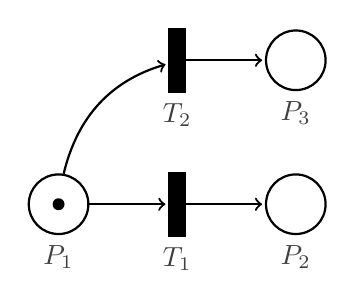
\begin{tikzpicture}[thick,
    every transition/.style={fill=black,minimum width=2mm, minimum height=8mm},
    every label/.style={black!75}]

% Place & transitions
\node[  place,
        label=below:$P_1$,
        tokens=1
    ] (place1) at (0,0) {};
\node[  transition,
        label=below:$T_1$,
        right=of place1,
    ] (trans1) {};
\node[  place,
        label=below:$P_2$,
        right=of trans1
    ] (place2) {};
\node[  transition,
        label=below:$T_2$,
        above=of trans1,
    ] (trans2) {};
\node[  place,
        label=below:$P_3$,
        right=of trans2
    ] (place3) {};
% Arcs
\draw[thick] (place1) edge[post] (trans1)
    (trans1) edge[post] (place2);
\draw[thick] (place1) edge[post, bend left] (trans2)
    (trans2) edge[post] (place3);

\end{tikzpicture}

\end{document}
